% --------------------------------------------------------------
%                         Template
% --------------------------------------------------------------

\documentclass[10pt]{article} %draft = show box warnings
\usepackage[a4paper, total={6.5in,10.2in}]{geometry} % Flexible and complete interface to document dimensions
\usepackage[utf8]{inputenc} % Accept different input encodings [utf8]
\usepackage[T1]{fontenc}    % Standard package for selecting font encodings
\usepackage{lmodern} % Good looking T1 font\usepackage{tikz}


% --------------------------------------------------------------
%                       Packages
% --------------------------------------------------------------
\usepackage{float} % Improved interface for floating objects
\usepackage{amsmath,amsthm,amssymb} % American Mathematics Society facilities
\usepackage[linktoc=all]{hyperref} % create hyperlinks
\usepackage{graphicx,booktabs,array}
\usepackage{subcaption}
\usepackage{xcolor}
\usepackage{tikz}
\usepackage{algorithmicx}
\usepackage{algorithm}
\usepackage{algpseudocode}
\usepackage[framemethod=TikZ]{mdframed}
\usepackage{epstopdf}

% --------------------------------------------------------------
%                       Exercise Env
% --------------------------------------------------------------

\newtheoremstyle{problemstyle}% name of the style to be used
  {20pt}% measure of space to leave above the theorem. E.g.: 3pt
  {3pt}% measure of space to leave below the theorem. E.g.: 3pt
  {}% name of font to use in the body of the theorem
  {}% measure of space to indent
  {}% name of head font
  {}% punctuation between head and body
  { }% space after theorem head; " " = normal interword space
  {\bfseries{Q\thmnumber{#2}.}}% Manually specify head
    
\theoremstyle{problemstyle}
\newtheorem{question}{\arabic{question}}

% --------------------------------------------------------------
%                       Colors
% --------------------------------------------------------------
\definecolor{face1}{RGB}{253,224,224}
\definecolor{face2}{RGB}{252,191,191}
\definecolor{face3}{RGB}{250,129,129}
\definecolor{face4}{RGB}{252,162,162}
\definecolor{face5}{RGB}{252, 210, 191}
\definecolor{comment}{RGB}{0, 128, 0}
% --------------------------------------------------------------
%                       Document
% --------------------------------------------------------------
\begin{document}
% --------------------------------------------------------------
%                       Header
% --------------------------------------------------------------
\noindent
\normalsize\textbf{Topological Data Analysis} \hfill \textbf{École Polytechnique}\\
\normalsize\textbf{INF556} \hfill \textbf{\today}\vspace{10pt}
\centerline{\Large }\vspace{5pt}
\centerline{\Large \textbf{TD 5 - Topological Persistence}}\vspace{8pt}
\centerline{Lucas Lugão Guimarães -- \texttt{lucas.lugao-guimaraes@polytechnique.edu}  }
\centerline{Alexandre Ribeiro João Macedo --  \texttt{alexandre.macedo@polytechnique.edu}}
\vspace{20pt}

% --------------------------------------------------------------
%                       Answers
% --------------------------------------------------------------
\begin{question} %Q1
The code of this implementation is attached in the final submission of this TD.
\end{question}

\begin{question} %Q2
The reduction algorithm already have the complexity requested in \hyperref[q:3]{question \ref*{q:3}} where we give an explanation for this complexity.
\end{question}

\begin{question} %Q3
\label{q:3}
The reduction algorithm can be seen bellow:
\end{question}

\begin{algorithm}
\caption{Reduction}
\begin{algorithmic}[1]
\State \textbf{let} $ R $ be a list of $m$ ordered sets representing the $\partial$ boundary matrix
\State \textbf{let} $P$ be an array of size $m$
\State $P \gets [-1,\dots,-1]$
\For {$j \gets 0$ \textbf{to} $m-1$}
	\While{$R[j]$ \textbf{is not empty}}
		\State $pivot \gets max(R[j])$ {\hfill \color{comment} the max function is $O(1)$ since $R[j]$ represents a ordered set.}
		\If{$pivot \geq 0$}
			\State {$R[j] \gets R[j] \ominus R[pivot]$}
		\Else
			\State \textbf{break}
		\EndIf
	\EndWhile
	\If{$R[j]$ \textbf{is empty}}
		\State {$pivots[max(R[j])] \gets j$}
	\EndIf
\EndFor
\end{algorithmic}
\end{algorithm}

In this implementation we can see two explicit loops in the lines 4 and 5 and an implicit one in the symmetrical difference at line 8. The first one obviously finishes after $m$ steps. The second one will continue to run while there is still ones in the $j$-th column to be eliminated, that means that it will run for at most $m$ steps (usually this number is much smaller due to the matrix sparsity). The last loop is the symmetrical difference of two given columns, this operation takes $O(m)$ steps as well. Hence, the given algorithm takes $O(m^3)$ to finish as requested.
\begin{question} %Q4

The function used to calculate the barcode is explained in the pseudocode below:
\end{question}

\begin{algorithm}[H]
\caption{Barcode}
\begin{algorithmic}[1]
\State \textbf{let} $F$ be an array of simplices representing the filtration
\State \textbf{let} $R$ be an array of $m$ ordered sets representing the reduced $\partial$ boundary matrix
\State \textbf{let} $P$ be an array of size $m$
\State \textbf{let} $B$ be a list representing the barcode
\State $P \gets [false,\dots,false]$
\For {$j \gets 0$ \textbf{to} $m-1$}
	\If{$R[j]$ \textbf{is not empty}}
		\State $P[max(R[j])] \gets true$ 
	\EndIf
\EndFor
\For {$j \gets 0$ \textbf{to} $m-1$}
	\If{$R[j]$ \textbf{is not empty}}
	    \State $birth \gets max(R[j])$
	    \State $death \gets j$
		\State $B.add([F[birth].dim, F[birth].val, F[death].val])$
	\Else
	    \If {\textbf{not} $P[j]$}
    		\State $B.add([F[j].dim, F[j].val, \infty])$
    	\EndIf
	\EndIf
\EndFor
\end{algorithmic}
\end{algorithm}
As in its implementation in C++ it has complexity $O(m)$ in time and space.
\begin{question} %Q5
The figures below show one possible filtration for the Moebius band, the torus, the Klein bottle, the projective plane, the d-sphere and the d-ball. For the d-ball, we only show the triangulations for d $\leq$ 3 and for the d-sphere, we only show the triangulation for d $\leq$ 2 due to the complexity or impossibility of representing the drawing for higher values of d. In \hyperref[q:6]{question \ref*{q:6}}, we show the bar codes for some of the filtrations.

\begin{figure}[H]
\centering
   \begin{subfigure}{0.3\linewidth}
	   	\begin{mdframed}[roundcorner=10pt]
	   		\centering
	   		\begin{tikzpicture}[every node/.style={circle, draw, inner sep=1.5pt},scale =0.9]
% Points
\node[label={[label distance=1pt]90: \tiny 1}] (l1) at (-2,1) {};
\node[label={[label distance=1pt]-90: \tiny 1}] (r1) at (2,0) {};
\node[label={[label distance=1pt]-90: \tiny 2}] (l2) at (-2,0) {};
\node[label={[label distance=1pt]90: \tiny 2}] (r2) at (2,1) {};
\node[label={[label distance=1pt]-90: \tiny 3}] (3) at (-1,0) {};
\node[label={[label distance=1pt]-90: \tiny 4}] (4) at (1,0) {};
\node[label={[label distance=1pt]90: \tiny 5}] (5) at (0,1) {};
\end{tikzpicture}
	   	\end{mdframed}
	   	\caption{0-simplexes}
	    \label{fig:mb-0-simplex} 
    \end{subfigure}
     \hfill
	\begin{subfigure}{0.3\linewidth}
	   	\begin{mdframed}[roundcorner=10pt]
	   		\centering
			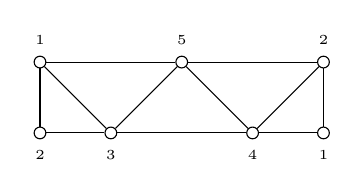
\begin{tikzpicture}[every node/.style={circle, draw, inner sep=1.5pt}, scale=0.9]
% Points
\node[label={[label distance=1pt]90: \tiny 1}] (l1) at (-2,1) {};
\node[label={[label distance=1pt]-90: \tiny 1}] (r1) at (2,0) {};
\node[label={[label distance=1pt]-90: \tiny 2}] (l2) at (-2,0) {};
\node[label={[label distance=1pt]90: \tiny 2}] (r2) at (2,1) {};
\node[label={[label distance=1pt]-90: \tiny 3}] (3) at (-1,0) {};
\node[label={[label distance=1pt]-90: \tiny 4}] (4) at (1,0) {};
\node[label={[label distance=1pt]90: \tiny 5}] (5) at (0,1) {};

%Lines
\draw (l1) -- (l2);
\draw (l1) -- (3);
\draw (l1) -- (5);
\draw (l2) -- (3);
\draw (3) -- (4);
\draw (3) -- (5);
\draw (5) -- (r2);
\draw (5) -- (4);
\draw (4) -- (r1);
\draw (4) -- (r2);
\draw (r1) -- (r2);
\end{tikzpicture}
		\end{mdframed}
		\caption{1-simplexes}
		\label{fig:mb-1-simplex} 
	\end{subfigure}
	\hfill
	\begin{subfigure}[H]{0.3\linewidth}
   		\begin{mdframed}[roundcorner=10pt]
   			\centering
   			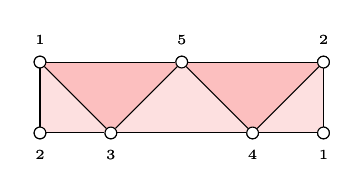
\begin{tikzpicture}[every node/.style={circle, draw, inner sep=1.5pt, fill=white}, scale=0.9]
% Points
\node[label={[label distance=1pt]90: \tiny 1}] (l1) at (-2,1) {};
\node[label={[label distance=1pt]-90: \tiny 1}] (r1) at (2,0) {};
\node[label={[label distance=1pt]-90: \tiny 2}] (l2) at (-2,0) {};
\node[label={[label distance=1pt]90: \tiny 2}] (r2) at (2,1) {};
\node[label={[label distance=1pt]-90: \tiny 3}] (3) at (-1,0) {};
\node[label={[label distance=1pt]-90: \tiny 4}] (4) at (1,0) {};
\node[label={[label distance=1pt]90: \tiny 5}] (5) at (0,1) {};

%Faces
\fill[color=face1] (l1.center) -- (l2.center) -- (3.center);
\fill[color=face2] (l1.center) -- (5.center) -- (3.center);
\fill[color=face1] (3.center) -- (5.center) -- (4.center);
\fill[color=face2] (5.center) -- (4.center) -- (r2.center);
\fill[color=face1] (4.center) -- (r2.center) -- (r1.center);

%Lines
\draw (l1) -- (l2);
\draw (l1) -- (3);
\draw (l1) -- (5);
\draw (l2) -- (3);
\draw (3) -- (4);
\draw (3) -- (5);
\draw (5) -- (r2);
\draw (5) -- (4);
\draw (4) -- (r1);
\draw (4) -- (r2);
\draw (r1) -- (r2);

% Points
\node[label={[label distance=1pt]90: \tiny 1}] (l1) at (-2,1) {};
\node[label={[label distance=1pt]-90: \tiny 1}] (r1) at (2,0) {};
\node[label={[label distance=1pt]-90: \tiny 2}] (l2) at (-2,0) {};
\node[label={[label distance=1pt]90: \tiny 2}] (r2) at (2,1) {};
\node[label={[label distance=1pt]-90: \tiny 3}] (3) at (-1,0) {};
\node[label={[label distance=1pt]-90: \tiny 4}] (4) at (1,0) {};
\node[label={[label distance=1pt]90: \tiny 5}] (5) at (0,1) {};
\end{tikzpicture}
   		\end{mdframed}
   		\caption{2-simplexes}
   		\label{fig:mb-2-simplex}
	\end{subfigure}
\centering
\caption{One possible filtration for the Moebius band.}
\label{fig:mb}
\end{figure}

\begin{figure}[H]
	\centering
	\begin{subfigure}{0.3\linewidth}
		
		\begin{mdframed}[roundcorner=10pt]
			\centering
			\begin{tikzpicture}[every node/.style={circle, draw, inner sep=1.5pt}]
% Points
\node[label={[label distance=1pt]180: \tiny 4}] (l4) at (0,0) {};
\node[label={[label distance=1pt]180: \tiny 5}] (l5) at (0,-1) {};
\node[label={[label distance=1pt]120: \tiny 1}] (lu1) at (0,1) {};
\node[label={[label distance=1pt]-120: \tiny 1}] (ld1) at (0,-2) {};
\node[label={[label distance=1pt]60: \tiny 6}] (5) at (1,0) {};
\node[label={[label distance=1pt]90: \tiny 2}] (u2) at (1,1) {};
\node[label={[label distance=1pt]60: \tiny 8}] (8) at (1,-1) {};
\node[label={[label distance=1pt]-90: \tiny 2}] (d2) at (1,-2) {};
\node[label={[label distance=1pt]60: \tiny 7}] (6) at (2,0) {};
\node[label={[label distance=1pt]90: \tiny 3}] (u3) at (2,1) {};
\node[label={[label distance=1pt]60: \tiny 9}] (9) at (2,-1) {};
\node[label={[label distance=1pt]-90: \tiny 3}] (d3) at (2,-2) {};
\node[label={[label distance=1pt]0: \tiny 4}] (r4) at (3,0) {};
\node[label={[label distance=1pt]60: \tiny 1}] (ru1) at (3,1) {};
\node[label={[label distance=1pt]0: \tiny 5}] (r5) at (3,-1) {};
\node[label={[label distance=1pt]-60: \tiny 1}] (rd1) at (3,-2) {};
\end{tikzpicture}
		\end{mdframed}
		\caption{0-simplexes}
		\label{fig:to-0-simplex} 
	\end{subfigure}
	\hfill
	\begin{subfigure}{0.3\linewidth}
		\begin{mdframed}[roundcorner=10pt]
			\centering
			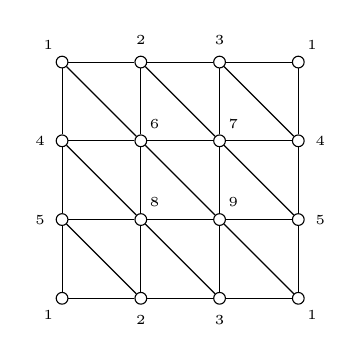
\begin{tikzpicture}[every node/.style={circle, draw, inner sep=1.5pt}]

% Points
\node[label={[label distance=1pt]180: \tiny 4}] (l4) at (0,0) {};
\node[label={[label distance=1pt]180: \tiny 5}] (l5) at (0,-1) {};
\node[label={[label distance=1pt]120: \tiny 1}] (lu1) at (0,1) {};
\node[label={[label distance=1pt]-120: \tiny 1}] (ld1) at (0,-2) {};
\node[label={[label distance=1pt]60: \tiny 6}] (6) at (1,0) {};
\node[label={[label distance=1pt]90: \tiny 2}] (u2) at (1,1) {};
\node[label={[label distance=1pt]60: \tiny 8}] (8) at (1,-1) {};
\node[label={[label distance=1pt]-90: \tiny 2}] (d2) at (1,-2) {};
\node[label={[label distance=1pt]60: \tiny 7}] (7) at (2,0) {};
\node[label={[label distance=1pt]90: \tiny 3}] (u3) at (2,1) {};
\node[label={[label distance=1pt]60: \tiny 9}] (9) at (2,-1) {};
\node[label={[label distance=1pt]-90: \tiny 3}] (d3) at (2,-2) {};
\node[label={[label distance=1pt]0: \tiny 4}] (r4) at (3,0) {};
\node[label={[label distance=1pt]60: \tiny 1}] (ru1) at (3,1) {};
\node[label={[label distance=1pt]0: \tiny 5}] (r5) at (3,-1) {};
\node[label={[label distance=1pt]-60: \tiny 1}] (rd1) at (3,-2) {};

%Lines
\draw (lu1) -- (u2);
\draw (lu1) -- (l4);
\draw (lu1) -- (6);
\draw (u2) -- (u3);
\draw (u2) -- (6);
\draw (u2) -- (7);
\draw (u3) -- (ru1);
\draw (u3) -- (7);
\draw (u3) -- (r4);
\draw (l4) -- (l5);
\draw (l4) -- (6);
\draw (l4) -- (8);
\draw (6) -- (8);
\draw (6) -- (7);
\draw (6) -- (9);
\draw (7) -- (9);
\draw (7) -- (r5);
\draw (l5) -- (8);
\draw (l5) -- (ld1);
\draw (l5) -- (d2);
\draw (8) -- (d2);
\draw (8) -- (9);
\draw (8) -- (d3);
\draw (9) -- (d3);
\draw (9) -- (r5);
\draw (9) -- (rd1);
\draw (ru1) -- (r4);
\draw (7) -- (r4);
\draw (r4) -- (r5);
\draw (r5) -- (rd1);
\draw (ld1) -- (d2);
\draw (d2) -- (d3);
\draw (d3) -- (rd1);
\end{tikzpicture}
		\end{mdframed}
		\caption{1-simplexes}
		\label{fig:to-1-simplex} 
	\end{subfigure}
	\hfill
	\begin{subfigure}[H]{0.3\linewidth}
		\centering
		\begin{mdframed}[roundcorner=10pt]
			\centering
			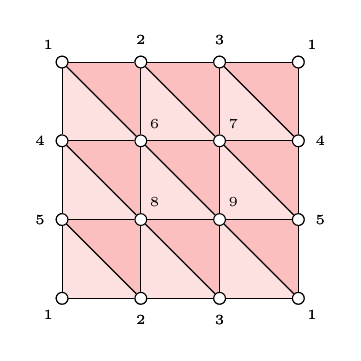
\begin{tikzpicture}[every node/.style={circle, draw, inner sep=1.5pt,fill=white}]
% Points
\node[label={[label distance=1pt]180: \tiny 4}] (l4) at (0,0) {};
\node[label={[label distance=1pt]180: \tiny 5}] (l5) at (0,-1) {};
\node[label={[label distance=1pt]120: \tiny 1}] (lu1) at (0,1) {};
\node[label={[label distance=1pt]-120: \tiny 1}] (ld1) at (0,-2) {};
\node[label={[label distance=1pt]60: \tiny 6}] (6) at (1,0) {};
\node[label={[label distance=1pt]90: \tiny 2}] (u2) at (1,1) {};
\node[label={[label distance=1pt]60: \tiny 8}] (8) at (1,-1) {};
\node[label={[label distance=1pt]-90: \tiny 2}] (d2) at (1,-2) {};
\node[label={[label distance=1pt]60: \tiny 7}] (7) at (2,0) {};
\node[label={[label distance=1pt]90: \tiny 3}] (u3) at (2,1) {};
\node[label={[label distance=1pt]60: \tiny 9}] (9) at (2,-1) {};
\node[label={[label distance=1pt]-90: \tiny 3}] (d3) at (2,-2) {};
\node[label={[label distance=1pt]0: \tiny 4}] (r4) at (3,0) {};
\node[label={[label distance=1pt]60: \tiny 1}] (ru1) at (3,1) {};
\node[label={[label distance=1pt]0: \tiny 5}] (r5) at (3,-1) {};
\node[label={[label distance=1pt]-60: \tiny 1}] (rd1) at (3,-2) {};

%Faces
\fill[color=face1] (lu1.center) -- (l4.center) -- (6.center);
\fill[color=face2] (lu1.center) -- (u2.center) -- (6.center);
\fill[color=face1] (u2.center) -- (6.center) -- (7.center);
\fill[color=face2] (u2.center) -- (u3.center) -- (7.center);
\fill[color=face1] (u3.center) -- (7.center) -- (r4.center);
\fill[color=face2] (u3.center) -- (ru1.center) -- (r4.center);
\fill[color=face1] (l4.center) -- (l5.center) -- (8.center);
\fill[color=face2] (l4.center) -- (6.center) -- (8.center);
\fill[color=face1] (6.center) -- (8.center) -- (9.center);
\fill[color=face2] (6.center) -- (7.center) -- (9.center);
\fill[color=face1] (7.center) -- (9.center) -- (r5.center);
\fill[color=face2] (7.center) -- (r4.center) -- (r5.center);
\fill[color=face1] (l5.center) -- (ld1.center) -- (d2.center);
\fill[color=face2] (l5.center) -- (8.center) -- (d2.center);
\fill[color=face1] (8.center) -- (d2.center) -- (d3.center);
\fill[color=face2] (8.center) -- (d3.center) -- (9.center);
\fill[color=face1] (9.center) -- (d3.center) -- (rd1.center);
\fill[color=face2] (9.center) -- (rd1.center) -- (r5.center);

%Lines
\draw (lu1) -- (u2);
\draw (lu1) -- (l4);
\draw (lu1) -- (6);
\draw (u2) -- (u3);
\draw (u2) -- (6);
\draw (u2) -- (7);
\draw (u3) -- (ru1);
\draw (u3) -- (7);
\draw (u3) -- (r4);
\draw (l4) -- (l5);
\draw (l4) -- (6);
\draw (l4) -- (8);
\draw (6) -- (8);
\draw (6) -- (7);
\draw (6) -- (9);
\draw (7) -- (9);
\draw (7) -- (r5);
\draw (l5) -- (8);
\draw (l5) -- (ld1);
\draw (l5) -- (d2);
\draw (8) -- (d2);
\draw (8) -- (9);
\draw (8) -- (d3);
\draw (9) -- (d3);
\draw (9) -- (r5);
\draw (9) -- (rd1);
\draw (ru1) -- (r4);
\draw (7) -- (r4);
\draw (r4) -- (r5);
\draw (r5) -- (rd1);
\draw (ld1) -- (d2);
\draw (d2) -- (d3);
\draw (d3) -- (rd1);
% Points
\node[label={[label distance=1pt]180: \tiny 4}] (l4) at (0,0) {};
\node[label={[label distance=1pt]180: \tiny 5}] (l5) at (0,-1) {};
\node[label={[label distance=1pt]120: \tiny 1}] (lu1) at (0,1) {};
\node[label={[label distance=1pt]-120: \tiny 1}] (ld1) at (0,-2) {};
\node[label={[label distance=1pt]60: \tiny 6}] (6) at (1,0) {};
\node[label={[label distance=1pt]90: \tiny 2}] (u2) at (1,1) {};
\node[label={[label distance=1pt]60: \tiny 8}] (8) at (1,-1) {};
\node[label={[label distance=1pt]-90: \tiny 2}] (d2) at (1,-2) {};
\node[label={[label distance=1pt]60: \tiny 7}] (7) at (2,0) {};
\node[label={[label distance=1pt]90: \tiny 3}] (u3) at (2,1) {};
\node[label={[label distance=1pt]60: \tiny 9}] (9) at (2,-1) {};
\node[label={[label distance=1pt]-90: \tiny 3}] (d3) at (2,-2) {};
\node[label={[label distance=1pt]0: \tiny 4}] (r4) at (3,0) {};
\node[label={[label distance=1pt]60: \tiny 1}] (ru1) at (3,1) {};
\node[label={[label distance=1pt]0: \tiny 5}] (r5) at (3,-1) {};
\node[label={[label distance=1pt]-60: \tiny 1}] (rd1) at (3,-2) {};
\end{tikzpicture}
		\end{mdframed}
		\caption{2-simplexes}
		\label{fig:to-2-simplex}
	\end{subfigure}
	\centering
	\caption{One possible filtration for the torus.}
	\label{fig:to}
\end{figure}

\begin{figure}[H]
	\centering
	\begin{subfigure}{0.3\linewidth}
		\centering
		\begin{mdframed}[roundcorner=10pt]
			\centering
			\begin{tikzpicture}[every node/.style={circle, draw, inner sep=1.5pt}]
% Points
\node[label={[label distance=1pt]180: \tiny 4}] (l4) at (0,0) {};
\node[label={[label distance=1pt]180: \tiny 5}] (l5) at (0,-1) {};
\node[label={[label distance=1pt]120: \tiny 1}] (lu1) at (0,1) {};
\node[label={[label distance=1pt]-120: \tiny 1}] (ld1) at (0,-2) {};
\node[label={[label distance=1pt]60: \tiny 6}] (5) at (1,0) {};
\node[label={[label distance=1pt]90: \tiny 2}] (u2) at (1,1) {};
\node[label={[label distance=1pt]60: \tiny 8}] (8) at (1,-1) {};
\node[label={[label distance=1pt]-90: \tiny 2}] (d2) at (1,-2) {};
\node[label={[label distance=1pt]60: \tiny 7}] (6) at (2,0) {};
\node[label={[label distance=1pt]90: \tiny 3}] (u3) at (2,1) {};
\node[label={[label distance=1pt]60: \tiny 9}] (9) at (2,-1) {};
\node[label={[label distance=1pt]-90: \tiny 3}] (d3) at (2,-2) {};
\node[label={[label distance=1pt]0: \tiny 5}] (r4) at (3,0) {};
\node[label={[label distance=1pt]60: \tiny 1}] (ru1) at (3,1) {};
\node[label={[label distance=1pt]0: \tiny 4}] (r5) at (3,-1) {};
\node[label={[label distance=1pt]-60: \tiny 1}] (rd1) at (3,-2) {};
\end{tikzpicture}
		\end{mdframed}
		\caption{0-simplexes}
		\label{fig:kl-0-simplex} 
	\end{subfigure}
	\hfill
	\begin{subfigure}{0.3\linewidth}
		\centering
		\begin{mdframed}[roundcorner=10pt]
			\centering
			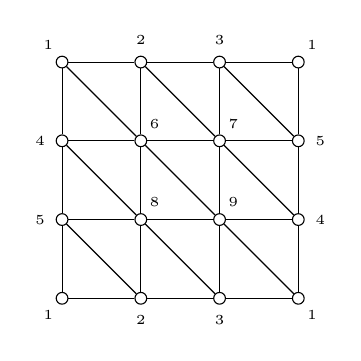
\begin{tikzpicture}[every node/.style={circle, draw, inner sep=1.5pt}]
% Points
% Points
\node[label={[label distance=1pt]180: \tiny 4}] (l4) at (0,0) {};
\node[label={[label distance=1pt]180: \tiny 5}] (l5) at (0,-1) {};
\node[label={[label distance=1pt]120: \tiny 1}] (lu1) at (0,1) {};
\node[label={[label distance=1pt]-120: \tiny 1}] (ld1) at (0,-2) {};
\node[label={[label distance=1pt]60: \tiny 6}] (6) at (1,0) {};
\node[label={[label distance=1pt]90: \tiny 2}] (u2) at (1,1) {};
\node[label={[label distance=1pt]60: \tiny 8}] (8) at (1,-1) {};
\node[label={[label distance=1pt]-90: \tiny 2}] (d2) at (1,-2) {};
\node[label={[label distance=1pt]60: \tiny 7}] (7) at (2,0) {};
\node[label={[label distance=1pt]90: \tiny 3}] (u3) at (2,1) {};
\node[label={[label distance=1pt]60: \tiny 9}] (9) at (2,-1) {};
\node[label={[label distance=1pt]-90: \tiny 3}] (d3) at (2,-2) {};
\node[label={[label distance=1pt]0: \tiny 5}] (r4) at (3,0) {};
\node[label={[label distance=1pt]60: \tiny 1}] (ru1) at (3,1) {};
\node[label={[label distance=1pt]0: \tiny 4}] (r5) at (3,-1) {};
\node[label={[label distance=1pt]-60: \tiny 1}] (rd1) at (3,-2) {};

%Lines
\draw (lu1) -- (u2);
\draw (lu1) -- (l4);
\draw (lu1) -- (6);
\draw (u2) -- (u3);
\draw (u2) -- (6);
\draw (u2) -- (7);
\draw (u3) -- (ru1);
\draw (u3) -- (7);
\draw (u3) -- (r4);
\draw (l4) -- (l5);
\draw (l4) -- (6);
\draw (l4) -- (8);
\draw (6) -- (8);
\draw (6) -- (7);
\draw (6) -- (9);
\draw (7) -- (9);
\draw (7) -- (r5);
\draw (l5) -- (8);
\draw (l5) -- (ld1);
\draw (l5) -- (d2);
\draw (8) -- (d2);
\draw (8) -- (9);
\draw (8) -- (d3);
\draw (9) -- (d3);
\draw (9) -- (r5);
\draw (9) -- (rd1);
\draw (ru1) -- (r4);
\draw (7) -- (r4);
\draw (r4) -- (r5);
\draw (r5) -- (rd1);
\draw (ld1) -- (d2);
\draw (d2) -- (d3);
\draw (d3) -- (rd1);
\end{tikzpicture}
		\end{mdframed}
		\caption{1-simplexes}
		\label{fig:kl-1-simplex} 
	\end{subfigure}
	\hfill
	\begin{subfigure}[H]{0.3\linewidth}
		\centering
		\begin{mdframed}[roundcorner=10pt]
			\centering
			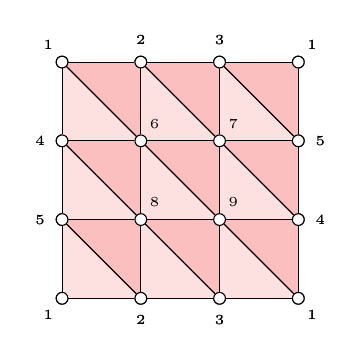
\begin{tikzpicture}[every node/.style={circle, draw, inner sep=1.5pt,fill=white}]
% Points
\node[label={[label distance=1pt]180: \tiny 4}] (l4) at (0,0) {};
\node[label={[label distance=1pt]180: \tiny 5}] (l5) at (0,-1) {};
\node[label={[label distance=1pt]120: \tiny 1}] (lu1) at (0,1) {};
\node[label={[label distance=1pt]-120: \tiny 1}] (ld1) at (0,-2) {};
\node[label={[label distance=1pt]60: \tiny 6}] (6) at (1,0) {};
\node[label={[label distance=1pt]90: \tiny 2}] (u2) at (1,1) {};
\node[label={[label distance=1pt]60: \tiny 8}] (8) at (1,-1) {};
\node[label={[label distance=1pt]-90: \tiny 2}] (d2) at (1,-2) {};
\node[label={[label distance=1pt]60: \tiny 7}] (7) at (2,0) {};
\node[label={[label distance=1pt]90: \tiny 3}] (u3) at (2,1) {};
\node[label={[label distance=1pt]60: \tiny 9}] (9) at (2,-1) {};
\node[label={[label distance=1pt]-90: \tiny 3}] (d3) at (2,-2) {};
\node[label={[label distance=1pt]0: \tiny 5}] (r4) at (3,0) {};
\node[label={[label distance=1pt]60: \tiny 1}] (ru1) at (3,1) {};
\node[label={[label distance=1pt]0: \tiny 4}] (r5) at (3,-1) {};
\node[label={[label distance=1pt]-60: \tiny 1}] (rd1) at (3,-2) {};

%Faces
\fill[color=face1] (lu1.center) -- (l4.center) -- (6.center);
\fill[color=face2] (lu1.center) -- (u2.center) -- (6.center);
\fill[color=face1] (u2.center) -- (6.center) -- (7.center);
\fill[color=face2] (u2.center) -- (u3.center) -- (7.center);
\fill[color=face1] (u3.center) -- (7.center) -- (r4.center);
\fill[color=face2] (u3.center) -- (ru1.center) -- (r4.center);
\fill[color=face1] (l4.center) -- (l5.center) -- (8.center);
\fill[color=face2] (l4.center) -- (6.center) -- (8.center);
\fill[color=face1] (6.center) -- (8.center) -- (9.center);
\fill[color=face2] (6.center) -- (7.center) -- (9.center);
\fill[color=face1] (7.center) -- (9.center) -- (r5.center);
\fill[color=face2] (7.center) -- (r4.center) -- (r5.center);
\fill[color=face1] (l5.center) -- (ld1.center) -- (d2.center);
\fill[color=face2] (l5.center) -- (8.center) -- (d2.center);
\fill[color=face1] (8.center) -- (d2.center) -- (d3.center);
\fill[color=face2] (8.center) -- (d3.center) -- (9.center);
\fill[color=face1] (9.center) -- (d3.center) -- (rd1.center);
\fill[color=face2] (9.center) -- (rd1.center) -- (r5.center);

%Lines
\draw (lu1) -- (u2);
\draw (lu1) -- (l4);
\draw (lu1) -- (6);
\draw (u2) -- (u3);
\draw (u2) -- (6);
\draw (u2) -- (7);
\draw (u3) -- (ru1);
\draw (u3) -- (7);
\draw (u3) -- (r4);
\draw (l4) -- (l5);
\draw (l4) -- (6);
\draw (l4) -- (8);
\draw (6) -- (8);
\draw (6) -- (7);
\draw (6) -- (9);
\draw (7) -- (9);
\draw (7) -- (r5);
\draw (l5) -- (8);
\draw (l5) -- (ld1);
\draw (l5) -- (d2);
\draw (8) -- (d2);
\draw (8) -- (9);
\draw (8) -- (d3);
\draw (9) -- (d3);
\draw (9) -- (r5);
\draw (9) -- (rd1);
\draw (ru1) -- (r4);
\draw (7) -- (r4);
\draw (r4) -- (r5);
\draw (r5) -- (rd1);
\draw (ld1) -- (d2);
\draw (d2) -- (d3);
\draw (d3) -- (rd1);
% Points
\node[label={[label distance=1pt]180: \tiny 4}] (l4) at (0,0) {};
\node[label={[label distance=1pt]180: \tiny 5}] (l5) at (0,-1) {};
\node[label={[label distance=1pt]120: \tiny 1}] (lu1) at (0,1) {};
\node[label={[label distance=1pt]-120: \tiny 1}] (ld1) at (0,-2) {};
\node[label={[label distance=1pt]60: \tiny 6}] (6) at (1,0) {};
\node[label={[label distance=1pt]90: \tiny 2}] (u2) at (1,1) {};
\node[label={[label distance=1pt]60: \tiny 8}] (8) at (1,-1) {};
\node[label={[label distance=1pt]-90: \tiny 2}] (d2) at (1,-2) {};
\node[label={[label distance=1pt]60: \tiny 7}] (7) at (2,0) {};
\node[label={[label distance=1pt]90: \tiny 3}] (u3) at (2,1) {};
\node[label={[label distance=1pt]60: \tiny 9}] (9) at (2,-1) {};
\node[label={[label distance=1pt]-90: \tiny 3}] (d3) at (2,-2) {};
\node[label={[label distance=1pt]0: \tiny 5}] (r4) at (3,0) {};
\node[label={[label distance=1pt]60: \tiny 1}] (ru1) at (3,1) {};
\node[label={[label distance=1pt]0: \tiny 4}] (r5) at (3,-1) {};
\node[label={[label distance=1pt]-60: \tiny 1}] (rd1) at (3,-2) {};
\end{tikzpicture}
		\end{mdframed}
		\caption{2-simplexes}
		\label{fig:kl-2-simplex}
	\end{subfigure}
	\centering
	\caption{One possible filtration for the Klein bottle.}
	\label{fig:kl}
\end{figure}

\begin{figure}[H]
	\centering
	\begin{subfigure}{0.32\linewidth}
		\begin{mdframed}[roundcorner=10pt]
			\centering
			\begin{tikzpicture}[every node/.style={circle, draw, inner sep=1.5pt,fill=white},scale=0.8]
% Points
\node[label={[label distance=1pt]90: \tiny 1}] (u1) at (0,1.5) {};
\node[label={[label distance=1pt]120: \tiny 4}] (4) at (0,0) {};
\node[label={[label distance=1pt]180: \tiny 3}] (l3) at (-2,0) {};
\node[label={[label distance=1pt]0: \tiny 2}] (r2) at (2,0) {};
\node[label={[label distance=1pt]180: \tiny 2}] (l2) at (-2,-1.5) {};
\node[label={[label distance=1pt]90: \tiny 6}] (6) at (-1,-1.5) {};
\node[label={[label distance=1pt]90: \tiny 5}] (5) at (1,-1.5) {};
\node[label={[label distance=1pt]0: \tiny 3}] (r3) at (2,-1.5) {};
\node[label={[label distance=1pt]-90: \tiny 1}] (d1) at (0,-3) {};
\end{tikzpicture}
		\end{mdframed}
		\caption{0-simplexes}
		\label{fig:pp-0-simplex} 
	\end{subfigure}
	\hfill
	\begin{subfigure}{0.32\linewidth}
		\begin{mdframed}[roundcorner=10pt]
			\centering
			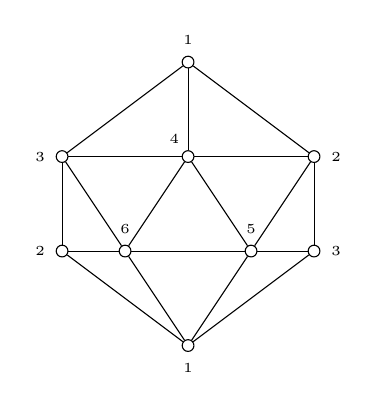
\begin{tikzpicture}[every node/.style={circle, draw, inner sep=1.5pt,fill=white},scale=0.8]
% Points
\node[label={[label distance=1pt]90: \tiny 1}] (u1) at (0,1.5) {};
\node[label={[label distance=1pt]120: \tiny 4}] (4) at (0,0) {};
\node[label={[label distance=1pt]180: \tiny 3}] (l3) at (-2,0) {};
\node[label={[label distance=1pt]0: \tiny 2}] (r2) at (2,0) {};
\node[label={[label distance=1pt]180: \tiny 2}] (l2) at (-2,-1.5) {};
\node[label={[label distance=1pt]90: \tiny 6}] (6) at (-1,-1.5) {};
\node[label={[label distance=1pt]90: \tiny 5}] (5) at (1,-1.5) {};
\node[label={[label distance=1pt]0: \tiny 3}] (r3) at (2,-1.5) {};
\node[label={[label distance=1pt]-90: \tiny 1}] (d1) at (0,-3) {};

%Lines
\draw (u1) -- (l3);
\draw (u1) -- (4);
\draw (u1) -- (r2);
\draw (l3) -- (4);
\draw (l3) -- (l2);
\draw (l3) -- (6);
\draw (4) -- (6);
\draw (4) -- (r2);
\draw (4) -- (5);
\draw (r2) -- (5);
\draw (r2) -- (r3);
\draw (l2) -- (6);
\draw (l2) -- (d1);
\draw (6) -- (5);
\draw (6) -- (d1);
\draw (5) -- (r3);
\draw (5) -- (d1);
\draw (r3) -- (d1);
\end{tikzpicture}
		 \end{mdframed}
		\caption{1-simplexes}
		\label{fig:pp-1-simplex} 
	\end{subfigure}
	\hfill
	\begin{subfigure}[H]{0.32\linewidth}
		\begin{mdframed}[roundcorner=10pt]
			\centering
			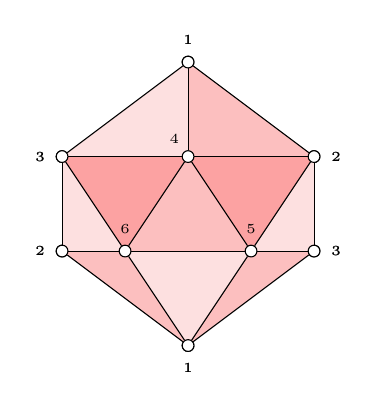
\begin{tikzpicture}[every node/.style={circle, draw, inner sep=1.5pt,fill=white}, scale=0.8]
% Points
\node[label={[label distance=1pt]90: \tiny 1}] (u1) at (0,1.5) {};
\node[label={[label distance=1pt]120: \tiny 4}] (4) at (0,0) {};
\node[label={[label distance=1pt]180: \tiny 3}] (l3) at (-2,0) {};
\node[label={[label distance=1pt]0: \tiny 2}] (r2) at (2,0) {};
\node[label={[label distance=1pt]180: \tiny 2}] (l2) at (-2,-1.5) {};
\node[label={[label distance=1pt]90: \tiny 6}] (6) at (-1,-1.5) {};
\node[label={[label distance=1pt]90: \tiny 5}] (5) at (1,-1.5) {};
\node[label={[label distance=1pt]0: \tiny 3}] (r3) at (2,-1.5) {};
\node[label={[label distance=1pt]-90: \tiny 1}] (d1) at (0,-3) {};

%Faces
\fill[color=face1] (u1.center) -- (l3.center) -- (4.center);
\fill[color=face2] (u1.center) -- (4.center) -- (r2.center);
\fill[color=face1] (l3.center) -- (l2.center) -- (6.center);
\fill[color=face4] (l3.center) -- (6.center) -- (4.center);
\fill[color=face2] (6.center) -- (4.center) -- (5.center);
\fill[color=face4] (4.center) -- (5.center) -- (r2.center);
\fill[color=face1] (5.center) -- (r3.center) -- (r2.center);
\fill[color=face2] (l2.center) -- (6.center) -- (d1.center);
\fill[color=face1] (6.center) -- (d1.center) -- (5.center);
\fill[color=face2] (d1.center) -- (5.center) -- (r3.center);

%Lines
\draw (u1) -- (l3);
\draw (u1) -- (4);
\draw (u1) -- (r2);
\draw (l3) -- (4);
\draw (l3) -- (l2);
\draw (l3) -- (6);
\draw (4) -- (6);
\draw (4) -- (r2);
\draw (4) -- (5);
\draw (r2) -- (5);
\draw (r2) -- (r3);
\draw (l2) -- (6);
\draw (l2) -- (d1);
\draw (6) -- (5);
\draw (6) -- (d1);
\draw (5) -- (r3);
\draw (5) -- (d1);
\draw (r3) -- (d1);

% Points
\node[label={[label distance=1pt]90: \tiny 1}] (u1) at (0,1.5) {};
\node[label={[label distance=1pt]120: \tiny 4}] (4) at (0,0) {};
\node[label={[label distance=1pt]180: \tiny 3}] (l3) at (-2,0) {};
\node[label={[label distance=1pt]0: \tiny 2}] (r2) at (2,0) {};
\node[label={[label distance=1pt]180: \tiny 2}] (l2) at (-2,-1.5) {};
\node[label={[label distance=1pt]90: \tiny 6}] (6) at (-1,-1.5) {};
\node[label={[label distance=1pt]90: \tiny 5}] (5) at (1,-1.5) {};
\node[label={[label distance=1pt]0: \tiny 3}] (r3) at (2,-1.5) {};
\node[label={[label distance=1pt]-90: \tiny 1}] (d1) at (0,-3) {};
\end{tikzpicture}
		\end{mdframed}
		\caption{2-simplexes}
		\label{fig:pp-2-simplex}
	\end{subfigure}
	\centering
	\caption{One possible filtration for the projective plane.}
	\label{fig:pp}
\end{figure}

\begin{figure}[H]
	\centering
	\begin{subfigure}{0.3\linewidth}
		\begin{mdframed}[roundcorner=10pt]
			\centering
			\begin{tikzpicture}[every node/.style={circle, draw, inner sep=1.5pt,fill=white}]
\filldraw[fill=white, draw=white] (-1,-1) rectangle (1,1);
\node[label={[label distance=1pt]180: \tiny 1}] (1) at (0,0) {};
\end{tikzpicture}
		\end{mdframed}
	
		\caption{0-ball. 100}
		\label{fig:0-ball} 
	\end{subfigure}
	\hfill
	\begin{subfigure}{0.3\linewidth}
		\centering
		\begin{mdframed}[roundcorner=10pt]
			\centering
			\begin{tikzpicture}[every node/.style={circle, draw, inner sep=1.5pt,fill=white}]
\filldraw[fill=white, draw=white] (-1,-1) rectangle (1,1);
\node[label={[label distance=1pt]180: \tiny 1}] (1) at (-0.5,0) {};
\node[label={[label distance=1pt]0: \tiny 2}] (2) at (0.5,0) {};
\end{tikzpicture}
		 \end{mdframed}
		\caption{0-sphere. 200}
		\label{fig:0-sphere} 
	\end{subfigure}
	\hfill
	\begin{subfigure}[H]{0.3\linewidth}
		\centering
		\begin{mdframed}[roundcorner=10pt]
			\centering
			\begin{tikzpicture}[every node/.style={circle, draw, inner sep=1.5pt,fill=white}]
\filldraw[fill=white, draw=white] (-1,-1) rectangle (1,1);
\node[label={[label distance=1pt]180: \tiny 1}] (1) at (-0.5,0) {};
\node[label={[label distance=1pt]0: \tiny 2}] (2) at (0.5,0) {};

\draw (1) -- (2);
\end{tikzpicture}
		\end{mdframed}
		\caption{1-ball. 100}
		\label{fig:1-ball}
	\end{subfigure}
	\\[\baselineskip]
	\begin{subfigure}{0.3\linewidth}
		\begin{mdframed}[roundcorner=10pt]
			\centering
			\begin{tikzpicture}[every node/.style={circle, draw, inner sep=1.5pt,fill=white}]
\filldraw[fill=white, draw=white] (-1,-0.5) rectangle (1,2.7);
\node[label={[label distance=1pt]210: \tiny 1}] (1) at (-1,0) {};
\node[label={[label distance=1pt]-30: \tiny 2}] (2) at (1,0) {};
\node[label={[label distance=1pt]90: \tiny 3}] (3) at (0,1.7) {};

\draw (1) -- (2);
\draw (2) -- (3);
\draw (1) -- (3);
\end{tikzpicture}
		\end{mdframed}
		\caption{1-sphere. 110}
		\label{fig:1-sphere} 
	\end{subfigure}
	\hfill
	\begin{subfigure}[H]{0.3\linewidth}
		\centering
		\begin{mdframed}[roundcorner=10pt]
			\centering
			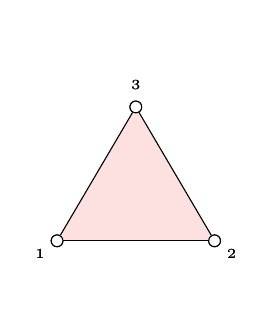
\begin{tikzpicture}[every node/.style={circle, draw, inner sep=1.5pt,fill=white}]
\filldraw[fill=white, draw=white] (-1,-0.5) rectangle (1,2.7);
\node[label={[label distance=1pt]210: \tiny 1}] (1) at (-1,0) {};
\node[label={[label distance=1pt]-30: \tiny 2}] (2) at (1,0) {};
\node[label={[label distance=1pt]90: \tiny 3}] (3) at (0,1.7) {};

\fill[color=face1] (1.center) -- (2.center) -- (3.center);

\draw (1) -- (2);
\draw (2) -- (3);
\draw (1) -- (3);

\node[label={[label distance=1pt]210: \tiny 1}] (1) at (-1,0) {};
\node[label={[label distance=1pt]-30: \tiny 2}] (2) at (1,0) {};
\node[label={[label distance=1pt]90: \tiny 3}] (3) at (0,1.7) {};
\end{tikzpicture}
		\end{mdframed}
		\caption{2-ball. 100}
		\label{fig:2-ball}
	\end{subfigure}
	\hfill
	\begin{subfigure}{0.3\linewidth}
		\begin{mdframed}[roundcorner=10pt]
			\centering
			% 2-sphere
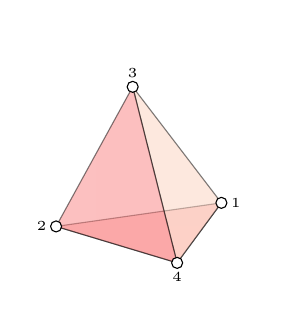
\begin{tikzpicture}[line join = round, line cap = round]
\filldraw[fill=white, draw=white] (-2,-0.5) rectangle (0,2);
\pgfmathsetmacro{\factor}{1/sqrt(2)};
\coordinate [label=right:\tiny 1] (1) at (-0.2,0,0.8*\factor);
\coordinate [label=left:\tiny 2] (2) at (-2,0,1.9*\factor);
\coordinate [label=above:\tiny 3] (3) at (-1,1.8,2*\factor);
\coordinate [label=below:\tiny 4] (4) at (0,0,3.6*\factor);


\draw[-, fill=face4, opacity=.5] (1)--(4)--(2)--cycle;
\draw[-, fill=face5, opacity=.5] (1) --(4)--(3)--cycle;
\draw[-, fill=face3, opacity=.5] (2)--(4)--(3)--cycle;

\draw[fill=white] (1) circle (2pt);
\draw[fill=white] (2) circle (2pt);
\draw[fill=white] (3) circle (2pt);
\draw[fill=white] (4) circle (2pt);
\end{tikzpicture}
		\end{mdframed}
		\caption{2-sphere. 101}
		\label{fig:2-sphere} 
	\end{subfigure}
	\\[\baselineskip]
	\begin{subfigure}[H]{0.3\linewidth}
		\begin{mdframed}[roundcorner=10pt]
		\centering
		% 3-ball
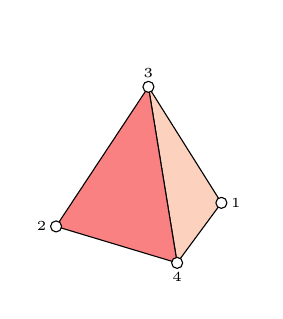
\begin{tikzpicture}[line join = round, line cap = round]
\filldraw[fill=white, draw=white] (-2,-0.5) rectangle (0,2);
\pgfmathsetmacro{\factor}{1/sqrt(2)};
\coordinate [label=right:\tiny 1] (1) at (-0.2,0,0.8*\factor);
\coordinate [label=left:\tiny 2] (2) at (-2,0,1.9*\factor);
\coordinate [label=above:\tiny 3] (3) at (-0.8,1.8,2*\factor);
\coordinate [label=below:\tiny 4] (4) at (0,0,3.6*\factor);

\draw[-, fill=face5] (1) --(4)--(3)--cycle;
\draw[-, fill=face3] (2)--(4)--(3)--cycle;

\draw[fill=white] (1) circle (2pt);
\draw[fill=white] (2) circle (2pt);
\draw[fill=white] (3) circle (2pt);
\draw[fill=white] (4) circle (2pt);
\end{tikzpicture}
		\end{mdframed}
		\caption{3-ball. 100}
		\label{fig:3-ball}
	\end{subfigure}
	\centering
	\caption{D-ball and d-sphere triangulations. The Betti numbers are given in the captions.}
	\label{fig:d}
\end{figure}

\end{question}

\begin{question} %Q6
For the computed barcodes, we can validate our results. For example, for the torus we saw that the number of Betti was 121, as we spected it to be. For the d-balls and d-spheres, we saw that it started by creating the points and the final Betti number was for the ball 100...0 and for the sphere 100...1.
% \begin{figure}[H]
% \centering
% 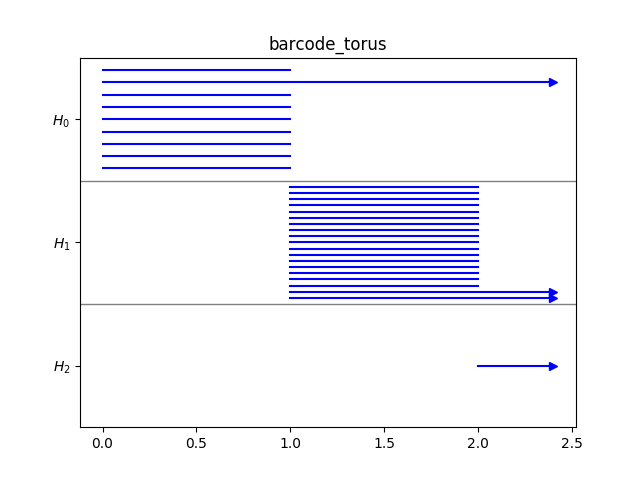
\includegraphics[scale=0.5]{torus.png}
% \caption{Barcode for the torus.}
% \end{figure}

\centering
\begin{figure}[H]
\begin{subfigure}[H]{0.4\linewidth}
\centering
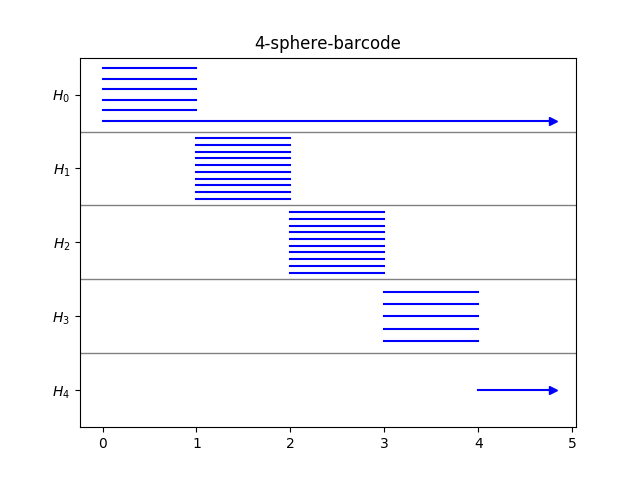
\includegraphics[scale=0.4]{4-ball.png}
\caption{Barcode for the 4-sphere.}
\end{subfigure}
\hfill
\begin{subfigure}[H]{0.4\linewidth}
\centering
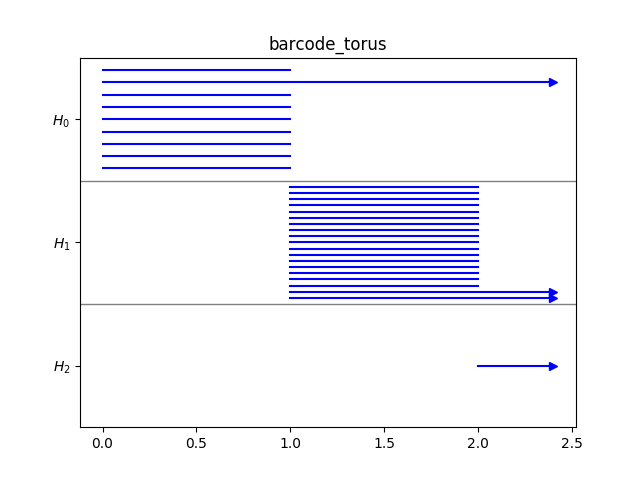
\includegraphics[scale=0.4]{torus.png}
\caption{Barcode for the torus.}
\end{subfigure}
\end{figure}

% \begin{figure}[H]
% \centering
% 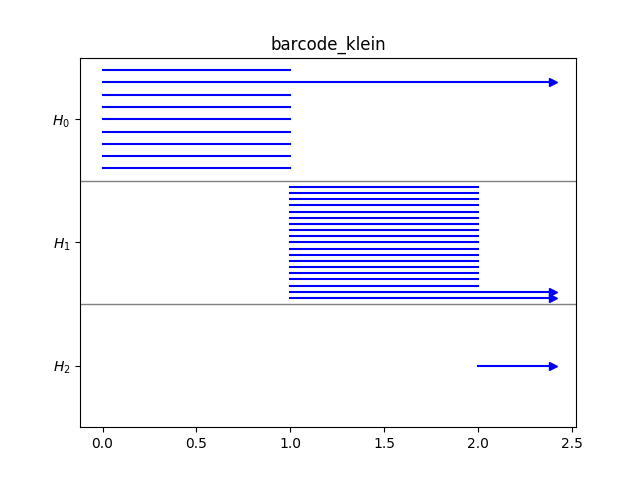
\includegraphics[scale=0.8]{klein.png}
% \caption{Barcode for the Klein bottle.}
% \end{figure}
\label{q:6}

\end{question}

\newpage
\begin{question} %Q7
\end{question}

\begin{figure}[H]
\centering
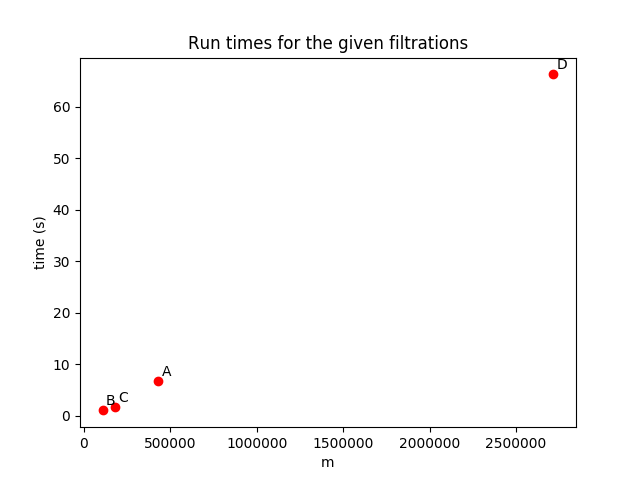
\includegraphics[scale=0.8]{plot_times.png}
\end{figure}
As can be seen in the picture above, the timings of the algorithm for each data set increases in a sub $O(m^3)$ this can be explained due to the sparse matrix representation. Anyway, if a dense approach had been chosen the timings would reflect this time complexity.

\begin{align*}
    m_A = 428643,\quad&t_A = 6.732\\
    m_B = 108161,\quad&t_B = 1.033\\
    m_C = 180347,\quad&t_C = 1.736\\
    m_D = 2716431,\quad&t_D = 66.260\\
\end{align*}

\begin{question} %Q8
\end{question}

    \begin{enumerate}
        \item[A)] The filtration A might show a 2-sphere. When the $H_1$ goes to zero $H_2$ goes to one. Then it keeps this $H_2$ for a while. When $H_2$ goes to zero, it means the filtration is "saturated".  
        \item[B)] For this filtration. We might think that it is composed by  tetrahedra. As the number of $H_2$ goes down as the time passes as they are filled. The $H_1$s represents triangles.
        \item[C)]The filtration B shows at times between 0 and 1 betti numbers (1,2,1) which corresponds possibly to a 2-torus or a klein bottle. Given that it then changes to a configuration with betti numbers (1,1,0), the one of a simple strip, it could indicate that in fact the original topological feature was of an torus. The noise in the filtration could indicate a Čech filtration of an point cloud generated from a 2-torus.
        \item[D)] This filtration shows some similarities whit the Klein bottle and the torus. Therefore, we can think of it as a filtration for a triangulation for one of these two.
    \end{enumerate}


\begin{thebibliography}{1}
	\bibitem{edel} %% To cite use \cite{example}
	Edelsbrunner, Herbert.
	\textit{A Short Course in Computational Geometry and Topology}. 
	Springer, 2014.
    
    \bibitem{toronto}
    \textit{Simplical Homology}. 
    \href{https://www.fields.utoronto.ca/programs/scientific/04-05/data_sets/parent.pdf}{Available here.}
    
    \bibitem{pplane}
    \textit{The Real Projective Plane Triangulated}.
    \href{http://www.math.jhu.edu/~jmb/note/rp2tri.pdf}{Available here.}
\end{thebibliography}

\end{document}
